% Copyright (c)  2005-2010 EDF-EADS-PHIMECA.
% Permission is granted to copy, distribute and/or modify this document
% under the terms of the GNU Free Documentation License, Version 1.2
% or any later version published by the Free Software Foundation;
% with no Invariant Sections, no Front-Cover Texts, and no Back-Cover
% Texts.  A copy of the license is included in the section entitled "GNU
% Free Documentation License".
\renewcommand{\filename}{docUC_StocProc_MonteCarlo.tex}
\renewcommand{\filetitle}{UC : Probability of a process event}

% \HeaderNNIILevel
% \HeaderIILevel
\HeaderIIILevel

\label{MonteCarloProcess}

\index{Stochastic Process!Monte Carlo  based on process}



The objective of this Use Case is to evaluate the probability of an event based on the  realizations of a stochastic process, using the Monte Carlo algorithm implemented in Open TURNS.\\

The Monte Carlo algooorithm is manimulated the same way as in the case where the event is based on a random variable independent of time. Details on the manipulation of the Monte Carlo algorithm and its results are presented in the Use Case  \ref{simuRes}. \\


Details on the Monte-Carlo algorithm may be found in the Reference Guide (\href{OpenTURNS_ReferenceGuide.pdf}{see files Reference Guide - Step C -- Estimating the probability of an event using Sampling} and files around).\\
Details on stochastic process may be found in the Reference Guide (\href{OpenTURNS_ReferenceGuide.pdf}{see Stochastic process}).\\
Details on each object may be found in the User Manual  (\href{OpenTURNS_UserManual_TUI.pdf}{see User Manual - EventProcess}).\\

\requirements{

  \begin{description}
  \item[$\bullet$] the domain : {\itshape myDomain}
  \item[type:] Domain
  \end{description}

  \begin{description}
  \item[$\bullet$] the process : {\itshape myProcess}
  \item[type:] Process
  \end{description}
}
{
  \begin{description}
  \item[$\bullet$] Event : {\itshape myEvent}
  \item[description:] use $Event$ with arguments $Domain$ and $Process$ and not $EventProcess$ 
  \item[type:] Event
  \end{description}

  \begin{description}
  \item[$\bullet$] the Monte-Carlo algorithm : {\itshape myMonteCarloAlgo}
  \item[type:] MonteCarlo
  \end{description}
}

\textspace\\
Python script for this Use Case :

\begin{lstlisting}
  # Create an event using a domain and a process
  myEvent = Event(myProcess, myDomain)


  # Create a Monte-Carlo algorithm based on myEvent
  myMonteCarloAlgo = MonteCarlo(myEvent)

  # Define the maximum number of simulations
  myMonteCarloAlgo.setMaximumOuterSampling(1000)

  # Define the block size
  myMonteCarloAlgo.setBlockSize(1000)

  # Define the maximum coefficient of variation
  myMonteCarloAlgo.setMaximumCoefficientOfVariation(0.001)

  # Run the algorithm
  myMonteCarloAlgo.run()

  # Get the result
  result = myMonteCarloAlgo.getResult()
  print result
\end{lstlisting}
\textspace\\

We applied the algorithm to the example presented in (\ref{EventProcess}) with  $10^4$ simulations, using the Monte-Carlo algorithm ($10^2$ $\times$ $10^3$ blocks).
Figure (\ref{mc_eventprocess_convergency}) draws the convergence graph of the estimator, with confidence level = $95\%$.
\begin{figure}[H]
    \begin{center}
      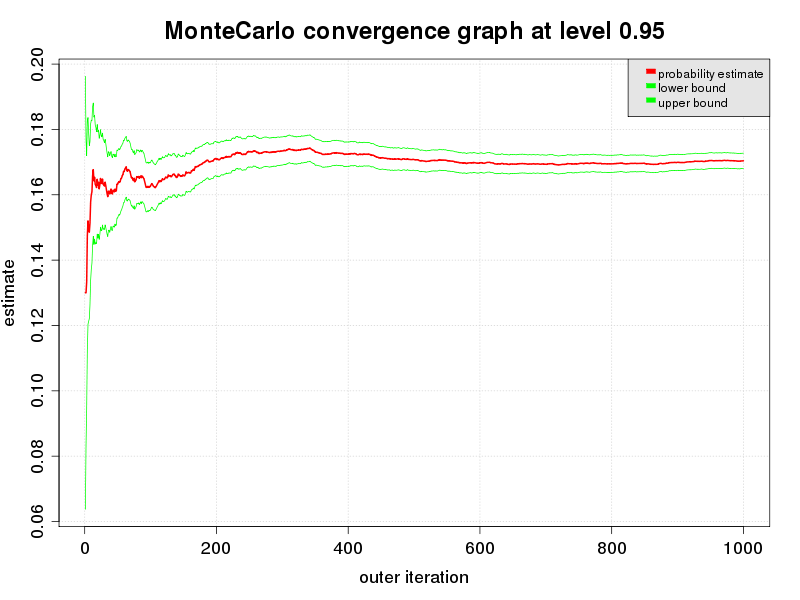
\includegraphics[width=7cm]{MonteCarloEventProcessConvergency.png}
      \caption{Convergence of the Monte-Carlo estimator based on a process event.}
      \label{mc_eventprocess_convergency}
    \end{center}
\end{figure}

The Monte-Carlo estimation of the probability is $p \simeq 0.1703$ and the condifence interval of order $95\%$ is $CI_{0.95}= [0.168, 0.173]$ .


